%%%%%%%%%%%%%%%%%%%%%%%%%%%%%%%%%%%%%%%%%
% University/School Laboratory Report
% LaTeX Template
% Version 3.1 (25/3/14)
%
% This template has been downloaded from:
% http://www.LaTeXTemplates.com
%
% Original author:
% Linux and Unix Users Group at Virginia Tech Wiki 
% (https://vtluug.org/wiki/Example_LaTeX_chem_lab_report)
%
% License:
% CC BY-NC-SA 3.0 (http://creativecommons.org/licenses/by-nc-sa/3.0/)
%
%%%%%%%%%%%%%%%%%%%%%%%%%%%%%%%%%%%%%%%%%

%----------------------------------------------------------------------------------------
%	PACKAGES AND DOCUMENT CONFIGURATIONS
%----------------------------------------------------------------------------------------

\documentclass{article}

\usepackage{graphicx} % Required for the inclusion of images
\usepackage{natbib} % Required to change bibliography style to APA
\usepackage{amsmath} % Required for some math elements 
\usepackage{amsthm}
\usepackage[hyphens]{url}
\usepackage{hyperref}
\usepackage{subcaption}
\usepackage{float}
\usepackage{array}
\usepackage{amssymb}
\usepackage{calrsfs}
\usepackage{pgfplots}
\pgfplotsset{width=10cm,compat=1.9}
\usepackage{bytefield}


\setlength\parindent{0pt} % Removes all indentation from paragraphs

\newtheorem*{remark}{Theorem}
\newtheorem*{definition}{Definition}

%----------------------------------------------------------------------------------------
%	DOCUMENT INFORMATION
%----------------------------------------------------------------------------------------

\title{Homework \#5 \\Telegram vs WhatsApp Security \\[0.2em]\small{}CNS Course Sapienza} % Title and subtitle

\author{Riccardo \textsc{Prinzivalle}, 1904064} % Author name

\date{November 30, 2020} % Date for the report

\begin{document}

\maketitle % Insert the title, author and date

%----------------------------------------------------------------------------------------
%	SECTION 0
%----------------------------------------------------------------------------------------

\section{Homework Goal}

This homework contains a basic introduction to Telegram and WhatsApp security, then a comparison of their security protocols (\textbf{MTProto} and \textbf{Signal} respectively), some past development and technical issues/vulnerabilities, and what it is possible to find about current threat and vulnerabilities.

%----------------------------------------------------------------------------------------
%	SECTION 1
%----------------------------------------------------------------------------------------

\section{Telegram Security basics}

Telegram uses a security protocol called MTProto, developed by the telegram team. It is a symmetric encryption protocol based on 256-bit symmetric AES encryption, 2048-bit RSA encryption and Diffie–Hellman key exchange. The protocol is divided in 3 layers:

\begin{itemize}
	\item \textbf{High-level} component which defines the method whereby API queries and responses are converted to binary messages.
	\item  \textbf{Cryptographic/authorization} layer which defines the method used to encrypt messages prior to being transmitted through the transport protocol.
	\item  \textbf{Transport} component, which defines the method for the client and the server to transmit messages over some other existing network protocol.
\end{itemize}

Let's analyze in the details every section. The high level component sees a client and a server exchanging messages inside a session, which is identified by a user key identifier (a particularity, the session is attached to the client instead of standard protocols such as http/s or tcp). The client can instantiate different connections to the server (the practicality of Telegram stands in the fact that one can open different sessions on many devices such as browsers without having to log in many times once one have the session active), and messages can be sent from one connection to the other and everything is synchronized server side. The low level message structure can be seen in fig. \ref{fig:tel_pack}.

\begin{figure}[H]
	\centering
	\begin{bytefield}[bitwidth=0.55em]{64}
		\bitheader{0,4,8,12,16,20,24,28,32,36,40,44,48,52,56,60,64} \\
		\begin{rightwordgroup}{encryption \\ header}
			\bitbox{64}{key identifier} \\
			\wordbox[tlr]{1}{message key} \\
			\wordbox[blr]{1}{128 bit} 
		\end{rightwordgroup} \\
		\\
		\begin{rightwordgroup}{message \\ header}
			\bitbox{64}{message identifier} \\
			\bitbox{64}{server salt}
		\end{rightwordgroup}
		\\
		\begin{rightwordgroup}{message \\ payload}
			\bitbox{32}{message sequence number} & \bitbox{32}{message length} \\
			\wordbox[tlr]{3}{message body (32 bit multiple)} \\
			\bitbox[blr]{32}{}
			& \bitbox{32}{type dependent parameters}
		\end{rightwordgroup} \\
	\end{bytefield}
	\caption{Telegram simplified packet structure}
	\label{fig:tel_pack}
\end{figure}

The message header is fixed for every message, the types of parameters does not change, and they are used by the encryption part, like message identifier and server salt.\newline
To be mentioned, all number are saved as little endian, with the exception of large numbers, such as those needed by RSA and DH which are stored as big endian due to openSSL compatibility.\newline
The encryption stuff can be identified in the upper part fig. \ref{fig:tel_pack}, it is added at the end of encryption as header of the encrypted message. The message is encrypted using a 256-bit key constituted by the message key and the user key and the encryption is performed with AES-256. The message key is defined as the hash using SHA256 on the message body, and taking the 128 middle resulting bits. The user key is generated from the authorization key: it is created once, when the client is first run on the device, and never changes, so this will expose all messages if that key is stolen (even from the device or from server side); different counter measures can be taken: 

\begin{itemize}
	\item Use session keys generated at every session using the Diffie Hellman exchange protocol
	\item Store the keys on the device and protect them with a password
	\item Protect all stored and cached data of the device with a password
\end{itemize}

All these measures cannot protect the user in the case where is the server that is violated or some government agency ask the keys for terrorism prevention (as example). The complete encryption scheme for every message can be seen in fig \ref{fig:MTProto}.

\begin{figure}[H]
	\centering
	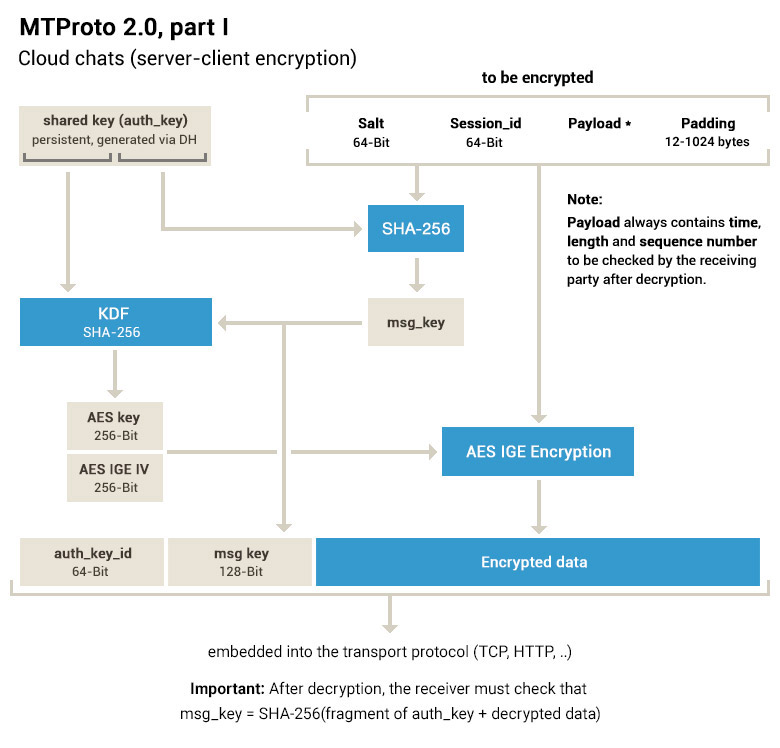
\includegraphics[width=0.9\textwidth]{images/mt_p1.jpg}
	\caption{MTProto}
	\label{fig:MTProto}
\end{figure}

The message identifier field is strictly related to time on the sender machine, and the receiver checks it with its time, so if there is a time divergence on sender or receiver message (here it is intended client/server communication and vice versa) then the receiver start to drop messages: in this case, the server (even if its time is not correct) will send a service message asking the client to synchronize its time with the server one. The time synchronization is simply defined as storing the difference between server and client time on client side. If the synchronization fails then the client must start a new session to continue the communication.\newline
The transport layer encapsulated the encrypted message with a secondary protocol header depending on specification of the message contained in the header, this allows to obtain additional services such as \textit{quick ack} or \textit{transport error}. The effective transport then relies on existent transport layer protocols as TCP, websockets or HTTP/S.\newline
This section has been developed using \cite{MTProto} and \cite{tel_wiki} as references.

%----------------------------------------------------------------------------------------
%	SECTION 3
%----------------------------------------------------------------------------------------

\section{WhatsApp Security Basics}

WhatsApp security relies on \textbf{Signal} protocol: it allows end-to-end encryption of every communication through the application. The protocol is based on the following steps:

\begin{itemize}
	\item Client registration and public keys exchange
	\item Encrypted session creation
	\item Message exchange using \textbf{Double Ratchet Algorithm} to generate a key for every message
\end{itemize}

When a new client is registered, some public keys are sent to the server who stores them: these keys are a \textit{public identity key}, a \textit{signed pre key} with its signature and a batch of \textit{one time pre keys}. These elements allow the server to uniquely identify a user identity.\newline
Every communication with a user is treated as an encrypted session: it is established at the first message exchanged and it does not change until no external factor changes the integrity of the session (this can happen due to a device change or an app reinstall). The session is created using the public keys of the receiver retrieved from the server and they are used to generate a master secret by "or" operation of different Diffie Hellman based on Elliptic Curves. The secret key is used by an hashed key derivation function to create a root key and some chain keys. If the recipient is not online at the time of the creation of the session, then the initiator includes the information to start the session with the first message sent, in order for the recipient to start the same encrypted session when he receives the messages.\newline
Every message sent through a session are encrypted by a message key using AES256 and HMAC-SHA256 for authentication. The message key changes for every message and it is ephemeral, so it is not possible to reconstruct an encrypted message from the session state. The key generation is based on the \textbf{Double Ratchet Algorithm}: it is based on HMAC-SHA256 to generate the single message key from the ratchet chain key and on the association of ECDH and HKDF to generate the new chain key and root key for the next message (these steps guarantee forward secrecy). This mechanism can cause delay in the messages and shift on the order of the original messages, but since every message is encrypted separately, it is not a problem. The Double ratchet scheme can be seen in fig. \ref{fig:doubleratchet}; the letters A and B are the message sent by Alice or Bob, and the number is the number of the message sent by one of them.

\begin{figure}[t]
	\centering
	\begin{subfigure}[b]{0.5\textwidth}
		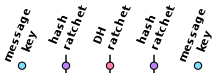
\includegraphics[width=1\linewidth]{images/doubleratchet_synt_header.png}
	\end{subfigure}
	\begin{subfigure}[b]{0.5\textwidth}
		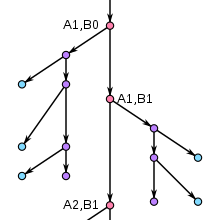
\includegraphics[width=1\linewidth]{images/doubleratchet_synt.png}
	\end{subfigure}
	\caption{Double Ratchet \cite{dr_scheme}}
	\label{fig:doubleratchet}
\end{figure}

The user can verify the end-to-end encryption keys to avoid a man-in-the-middle attack, the verification can be performed either by a QR code or by a 60 digit number, that the users must compare with the keys stored on their device to ensure no attack has been performed.\newline 
For what concerns the transport layer, WhatsApp uses the \textbf{Noise} protocol framework: this provides long time connections between the clients and the servers based on \textit{noise pipes} with Curve25519, AES-GCM, and SHA256.\newline
Unfortunately, I was not able to find images like fig. \ref{fig:MTProto} for WhatsApp; this is due to the nature of \textbf{Signal} protocol, which subdivides every step of security into separated applications, such as the Double Ratchet of fig. \ref{fig:doubleratchet}. This section is based on \cite{what_tech_paper}, \cite{what_medium}, \cite{what_wiki} and \cite{signal}.

%----------------------------------------------------------------------------------------
%	SECTION 4
%----------------------------------------------------------------------------------------

\section{Protocols comparison}


 
%----------------------------------------------------------------------------------------
%	SECTION 5
%----------------------------------------------------------------------------------------

\section{Past Evolution and Fixed Vulnerabilities}



%----------------------------------------------------------------------------------------
%	SECTION 6
%----------------------------------------------------------------------------------------

\section{Current Vulnerabilities and Security Threats}

%----------------------------------------------------------------------------------------
%	SECTION 7
%----------------------------------------------------------------------------------------

\section{Conclusion}

After this brief introduction on elliptic curves, it is obvious why they have been widely adopted in many cases of asymmetric encryption: they use less bits for the same level of security, so are more efficient to compute and their base concepts are easier to visualize. As suggested on section , EC can be easily used in hybrid encryption scheme, in the key exchange phase.

%----------------------------------------------------------------------------------------
%	BIBLIOGRAPHY
%----------------------------------------------------------------------------------------

\bibliographystyle{abbrv}

\bibliography{biblio}

%----------------------------------------------------------------------------------------


\end{document}